\documentclass[10pt,oneside,a4paper,openany]{book}

% --- 样式与宏包加载 (由 atlas_style.sty 统一管理) ---
\usepackage[UTF8, scheme=plain, fontset=fandol]{ctex}
\usepackage{atlas_style}

% --- 封面设计 (Times New Roman 风格) ---
\title{
    \vspace{2cm}
    \Huge \textbf{\textcolor{maintheme}{Deep Learning Mathematics Atlas}} \\
    \vspace{0.5cm}
    \Huge \textbf{\textcolor{maintheme}{深度学习数学图鉴}} \\
    \vspace{1cm}
    \Large \textit{\color{gray} 从 PyTorch 算子到 LaTeX 定义的硬核映射}
}
\author{\Large Antigravity \& Sisyphus \& 吴东泽}
\date{\vspace{1cm}\large \today \\ \vspace{0.5cm} \textbf{Edition 2.0}}

\begin{document}

\frontmatter
\maketitle

\tableofcontents
\newpage

\chapter*{前言 (Preface)}
\addcontentsline{toc}{chapter}{前言 (Preface)}

深度学习在工程上的辉煌胜利,往往掩盖了其底层严谨的数学逻辑。对于当今的 AI 开发者/刚入学的研究生/想做深度学习项目的人/对这方面感兴趣的本科生而言,我们正面临着一个普遍的困境:\textbf{黑盒化的陷阱}。

当我们敲下 \pyfunc{nn.Linear} 或 \pyfunc{nn.CrossEntropyLoss} 时,PyTorch 等现代框架以极其优雅的 API 替我们屏蔽了复杂的矩阵乘法、张量偏导与梯度流向。这种工程上的便利极大降低了入门门槛,但也让许多从业者逐渐沦为“调包侠”。

然而,当你试图复现一篇顶会论文(如 LLaMA 的旋转位置编码 RoPE,或是 Mamba 的选择性状态空间),当你遭遇训练过程中诡异的 NaN(梯度爆炸),或是当你想手写 CUDA 算子进行极限推理加速时,你会痛苦地发现:\textbf{仅仅读懂 Python 代码已经远远不够了}。

学术界的论文(Paper)是用纯粹的 LaTeX 数学语言写成的,而工程界的落地则是用 Python 和 C++ 堆砌的。这两者之间存在着巨大的认知鸿沟。本书正是为了打破这堵高墙,打造一块连接学术界与工程界的\textbf{罗塞塔石碑 (Rosetta Stone)}。

在此版本中,我们引入了全新的“左右对照”排版风格,旨在提供更直观的数学与代码映射体验。

\vspace{1cm}
\begin{flushright}
\textit{Antigravity \& Sisyphus \& 吴东泽} \\
2026年2月
\end{flushright}

\mainmatter

% --- 第一阶段:张量与基础 ---
\part{基石篇 (Foundations)}
\chapter{张量基础运算}
\label{ch:basics}

在深度学习中,张量(Tensor)是承载数据的基本容器。所有的复杂层最终都会分解为对这些多维数组的基础算子。

\marginpar{
    \centering
    \begin{tikzpicture}[scale=0.8, transform shape]
        \node[block] (A) {Tensor A};
        \node[block_orange, below=0.6cm of A] (OP) {Operation};
        \node[block_green, below=0.6cm of OP] (C) {Tensor C};
        \draw[conn] (A) -- (OP);
        \draw[arrow_blue] (OP) -- (C);
    \end{tikzpicture}
    \captionof{figure}{Tensor Operation Flow}
}

\section{逐元素运算 (Element-wise Operations)}

\subsection{Hadamard 乘积}
逐元素乘法是指两个形状相同的张量,对应位置的元素相乘。

\begin{rosetta}{逐元素乘法}
    \begin{equation}
        C = A \odot B \quad \text{其中 } C_{i,j} = A_{i,j} \times B_{i,j}
    \end{equation}
    \tcblower
    \pyfunc{torch.mul(A, B)} 或 \pyfunc{A * B}
\end{rosetta}

\subsection{幂运算}
对张量中的每一个分量求 $n$ 次幂。

\begin{rosetta}{幂运算}
    \begin{equation}
        y = x^n
    \end{equation}
    \tcblower
    \pyfunc{torch.pow(x, n)}
\end{rosetta}

\section{线性代数 (Linear Algebra)}

\subsection{矩阵乘法}
这是神经网络中线性变换的核心,常用于全连接层和注意力机制。

\begin{rosetta}{矩阵乘法}
    \begin{equation}
        C = AB \implies C_{i,j} = \sum_{k=1}^{n} A_{i,k}B_{k,j}
    \end{equation}
    \tcblower
    \pyfunc{torch.matmul(A, B)} 或 \pyfunc{A @ B}
\end{rosetta}

\subsection{转置}
交换张量的维度,在矩阵中通常指行与列的互换。

\begin{rosetta}{转置}
    \begin{equation}
        A_{i,j}^T = A_{j,i}
    \end{equation}
    \tcblower
    \pyfunc{tensor.T} 或 \pyfunc{tensor.t()}
\end{rosetta}

\section{统计规约 (Reduction)}

\subsection{L2 范数}
计算向量或矩阵的模长。

\begin{rosetta}{L2 范数}
    \begin{equation}
        \|\mathbf{x}\|_2 = \sqrt{\sum_{i=1}^{n} |x_i|^2}
    \end{equation}
    \tcblower
    \pyfunc{torch.norm(x, p=2)}
\end{rosetta}

\chapter{高级线性代数算子}
\label{ch:linalg_functions}

线性代数算子是深度学习底层的动力引擎。除了基础的矩阵乘法外,诸如奇异值分解(SVD)、特征值分解和爱因斯坦求和约定(Einsum)在现代模型压缩、稳定训练和高性能计算中扮演着至关重要的角色。

\section{矩阵分解 (Matrix Decomposition)}

\subsection{奇异值分解 (SVD)}
SVD 将任何矩阵分解为旋转、缩放和旋转三个过程。在深度学习中,常用于 LoRA 的权重初始化或模型压缩。

\begin{rosetta}{奇异值分解 (SVD)}
    \begin{equation}
        A = U \Sigma V^T
    \end{equation}
    其中:
    \begin{itemize}
        \item $U, V$ 是正交矩阵。
        \item $\Sigma$ 是对角矩阵,包含奇异值。
    \end{itemize}
    \tcblower
    \pyfunc{U, S, Vh = torch.linalg.svd(A)}
\end{rosetta}

\subsection{QR 分解}
QR 分解将矩阵分解为一个正交矩阵 $Q$ 和一个上三角矩阵 $R$。常用于数值稳定性要求极高的线性方程组求解。

\begin{rosetta}{QR 分解}
    \begin{equation}
        A = QR
    \end{equation}
    其中 $Q^T Q = I$,$R$ 为上三角。
    \tcblower
    \pyfunc{Q, R = torch.linalg.qr(A)}
\end{rosetta}

\section{矩阵属性与度量}

\subsection{行列式与逆}
虽然在反向传播中较少直接求逆,但在概率图模型或雅可比行列式计算中不可或缺。

\begin{rosetta}{行列式与逆矩阵}
    \begin{equation}
        \det(A) \cdot A^{-1} = \text{adj}(A)
    \end{equation}
    \tcblower
    \pyfunc{torch.linalg.det(A)} \\
    \pyfunc{torch.linalg.inv(A)}
\end{rosetta}

\subsection{矩阵范数 (Matrix Norm)}
用于度量矩阵的“大小”,在谱归一化(Spectral Normalization)中特指算子范数。

\begin{rosetta}{谱范数 (Spectral Norm)}
    \begin{equation}
        \|A\|_2 = \sigma_{\max}(A)
    \end{equation}
    即矩阵最大奇异值。
    \tcblower
    \pyfunc{torch.linalg.matrix\_norm(A, ord=2)}
\end{rosetta}

\section{高级张量约定}

\subsection{爱因斯坦求和约定 (Einsum)}
Einsum 是处理多维张量收缩的“瑞士军刀”,能以极简语法实现转置、乘法、迹和外积。

\begin{rosetta}{Einstein Summation}
    \begin{equation}
        C_{ij} = \sum_{k} A_{ik} B_{kj} \implies \texttt{ik,kj->ij}
    \end{equation}
    \tcblower
    \pyfunc{torch.einsum('ik,kj->ij', A, B)}
\end{rosetta}

\subsection{批量矩阵乘法 (BMM)}
在处理 Batch 数据(如 Attention 权重)时,高效处理前两个维度外的矩阵乘法。

\begin{rosetta}{Batch MatMul}
    \begin{equation}
        C_{b,i,j} = \sum_{k} A_{b,i,k} B_{b,k,j}
    \end{equation}
    \tcblower
    \pyfunc{torch.bmm(A, B)}
\end{rosetta}

\begin{center}
\begin{tikzpicture}[node distance=1.8cm, font=\sffamily\small]
    % SVD 示意图
    \node[data_node, fill=brandblue!10, minimum height=2cm] (A) {$A$};
    \node[right=1cm of A] (eq) {$=$};
    \node[data_node, right=1cm of eq, fill=brandorange!10, minimum height=2cm] (U) {$U$};
    \node[data_node, right=0.2cm of U, fill=brandgreen!10, minimum height=1cm, minimum width=1cm] (S) {$\Sigma$};
    \node[data_node, right=0.2cm of S, fill=brandblue!5, minimum width=2cm, minimum height=2cm] (V) {$V^T$};
    
    \node[layer_label, below=0.2cm of A] {Matrix};
    \node[layer_label, below=0.2cm of U] {Orthogonal};
    \node[layer_label, below=0.7cm of S] {Singular};
    \node[layer_label, below=0.2cm of V] {Orthogonal};
\end{tikzpicture}
\end{center}

\chapter{概率论基础 (Probability Foundations)}
\label{ch:probability}

概率论是深度学习处理不确定性、构建生成模型和设计损失函数的基石。所有的变分推断、扩散模型和信息论指标都建立在概率分布的基础之上。

\begin{notation}
\begin{itemize}
    \item $x$: Input tensor
    \item $\mu$: Mean
    \item $\mathbf{x}$: Input vector
\end{itemize}
\end{notation}

\mnote{$x$: Input tensor \\ $\mu$: Mean \\ $\mathbf{x}$: Input vector}
\section{常见概率分布 (Common Distributions)}

\subsection{正态分布 (Normal Distribution)}
正态分布(高斯分布)是自然界中最常见的连续概率分布,也是许多生成模型(如 VAE 和 Diffusion)的先验分布假设。

\begin{rosetta}{多元正态分布}
    \begin{equation}
        \mathcal{N}(\mathbf{x}|\boldsymbol{\mu}, \boldsymbol{\Sigma}) = \frac{1}{(2\pi)^{D/2}|\boldsymbol{\Sigma}|^{1/2}} \exp\left(-\frac{1}{2}(\mathbf{x}-\boldsymbol{\mu})^\top \boldsymbol{\Sigma}^{-1} (\mathbf{x}-\boldsymbol{\mu})\right)
    \end{equation}
    \tcblower
    \pyfunc{torch.distributions.MultivariateNormal(loc, covariance\_matrix)}
\end{rosetta}

\subsection{伯努利与多项式分布 (Bernoulli \& Categorical)}
离散分布常用于分类任务的标签建模。

\begin{rosetta}{分类分布 (Categorical Distribution)}
    \begin{equation}
        P(X=k) = p_k, \quad \sum_{k=1}^K p_k = 1
    \end{equation}
    \tcblower
    \pyfunc{torch.distributions.Categorical(probs=p)}
\end{rosetta}

\section{贝叶斯定理与变分推断 (Bayesian \& VI)}

贝叶斯定理是生成模型(如 VAE)处理潜在变量(Latent Variables)的核心理论。

\begin{rosetta}{贝叶斯定理 (Bayes' Theorem)}
    \begin{equation}
        P(Z|X) = \frac{P(X|Z)P(Z)}{P(X)}
    \end{equation}
    其中 $P(Z|X)$ 是后验,$P(X|Z)$ 是似然,$P(Z)$ 是先验。
    \tcblower
    在深度学习中,我们通常使用编码器 $q_\phi(Z|X)$ 来近似难以计算的真后验 $P(Z|X)$。
\end{rosetta}

\section{马尔可夫链 (Markov Chains)}
马尔可夫链描述了一个状态空间中经过从一个状态到另一个状态的转换的随机过程。该过程要求具备“无记忆”的性质(即马尔可夫性质)。

\begin{figure}[htbp]
    \centering
    \begin{tikzpicture}[
        node distance=2.5cm,
        state/.style={circle, draw=maintheme, thick, fill=maintheme!10, minimum size=1.2cm, align=center},
        arrow/.style={-stealth, thick, draw=black!70}
    ]
        \node[state] (S1) {$S_1$};
        \node[state, right of=S1, xshift=1.5cm] (S2) {$S_2$};
        \node[state, right of=S2, xshift=1.5cm] (S3) {$S_3$};

        \draw[arrow] (S1) edge[bend left] node[above] {$P_{12}$} (S2);
        \draw[arrow] (S2) edge[bend left] node[below] {$P_{21}$} (S1);
        \draw[arrow] (S2) edge[bend left] node[above] {$P_{23}$} (S3);
        \draw[arrow] (S3) edge[bend left] node[below] {$P_{32}$} (S2);
        
        \draw[arrow] (S1) edge[loop above] node[above] {$P_{11}$} (S1);
        \draw[arrow] (S2) edge[loop above] node[above] {$P_{22}$} (S2);
        \draw[arrow] (S3) edge[loop right] node[right] {$P_{33}$} (S3);
    \end{tikzpicture}
    \caption{简单的马尔可夫链状态转移图}
    \label{fig:markov_chain}
\end{figure}

马尔可夫性质的数学定义为:
\begin{equation}
    P(X_{n+1}=x | X_n=x_n, X_{n-1}=x_{n-1}, \dots, X_0=x_0) = P(X_{n+1}=x | X_n=x_n)
\end{equation}

\chapter{激活函数}
\label{ch:activations}

激活函数通过引入非线性变换,使得神经网络能够拟合极其复杂的函数分布。

\marginpar{
    \centering
    \begin{tikzpicture}[scale=0.8]
        \draw[->, gray] (-2,0) -- (2,0) node[right] {$x$};
        \draw[->, gray] (0,-1) -- (0,2) node[above] {$y$};
        \draw[thick, brandorange] (-1.5,0) -- (0,0) -- (1.5,1.5) node[right] {ReLU};
    \end{tikzpicture}
    \captionof{figure}{ReLU Function}
}

\begin{notation}
\begin{itemize}
    \item $x$: Input tensor
    \item $y$: Output label
    \item $\sigma$: Activation function
\end{itemize}
\end{notation}

\mnote{$x$: Input tensor \\ $y$: Output label \\ $\sigma$: Activation function}
\section{常用激活函数}

\subsection{ReLU (Rectified Linear Unit)}
ReLU 是深度学习中最常用的激活函数,因其计算简单且能有效缓解梯度消失问题。

\begin{rosetta}{ReLU 激活函数}
    \begin{equation}
        \text{ReLU}(x) = \max(0, x)
    \end{equation}
    \tcblower
    \pyfunc{torch.relu(x)} 或 \pyfunc{nn.ReLU()}
\end{rosetta}

\subsection{Sigmoid}
将输入映射到 $(0, 1)$ 区间,常用于二分类问题的概率预测。

\begin{rosetta}{Sigmoid 激活函数}
    \begin{equation}
        \sigma(x) = \frac{1}{1 + e^{-x}}
    \end{equation}
    \tcblower
    \pyfunc{torch.sigmoid(x)} 或 \pyfunc{nn.Sigmoid()}
\end{rosetta}

\subsection{Tanh (双曲正切)}
将输入映射到 $(-1, 1)$ 区间,输出均值为 0,在某些网络中比 Sigmoid 收敛更快。

\begin{rosetta}{Tanh 激活函数}
    \begin{equation}
        \tanh(x) = \frac{e^x - e^{-x}}{e^x + e^{-x}}
    \end{equation}
    \tcblower
    \pyfunc{torch.tanh(x)} 或 \pyfunc{nn.Tanh()}
\end{rosetta}

\subsection{Softmax}
常用于多分类任务的输出层,将一组向量转化为概率分布。

\begin{rosetta}{Softmax 函数}
    \begin{equation}
        \text{Softmax}(x_i) = \frac{e^{x_i}}{\sum_{j=1}^{C} e^{x_j}}
    \end{equation}
    \tcblower
    \pyfunc{torch.softmax(x, dim)}
\end{rosetta}


% --- 第二阶段:解剖神经网络 ---
\part{解剖篇 (Anatomy)}
\chapter{神经网络层}
\label{ch:layers}

神经网络层是参数的学习单元,它将基础算子封装成带有可学习权重的模块。

\marginpar{
    \centering
    \begin{tikzpicture}[scale=0.75, transform shape]
        % Input nodes
        \foreach \i in {1,2,3} {
            \node[neuron] (I\i) at (0,-\i*1.2) {};
        }
        % Hidden nodes
        \foreach \j in {1,2} {
            \node[active_neuron] (H\j) at (2,-0.6-\j*1.2) {};
        }
        % Connections
        \foreach \i in {1,2,3} {
            \foreach \j in {1,2} {
                \draw[conn] (I\i) -- (H\j);
            }
        }
        \node[layer_label] at (0,-4.5) {Input Layer};
        \node[layer_label] at (2,-4.5) {Linear Layer};
    \end{tikzpicture}
    \captionof{figure}{Linear Layer (Fully Connected)}
}

\section{线性变换与卷积}

\subsection{线性层 (Linear / Fully Connected)}
执行仿射变换,是多层感知机(MLP)的核心。

\begin{rosetta}{线性层}
    \begin{equation}
        \mathbf{y} = \mathbf{x} \mathbf{W}^T + \mathbf{b}
    \end{equation}
    其中 $\mathbf{W} \in \mathbb{R}^{out \times in}$ 是权重矩阵,$\mathbf{b} \in \mathbb{R}^{out}$ 是偏置向量。
    \tcblower
    \pyfunc{nn.Linear(in\_features, out\_features)}
\end{rosetta}

\subsection{2D 卷积层 (Convolutional Layer)}
卷积层通过局部连接和权值共享提取空间特征。注意:PyTorch 实际执行的是互相关运算。

\begin{rosetta}{2D 卷积}
    \textbf{输出尺寸计算公式}:
    \begin{equation}
        H_{out} = \left\lfloor \frac{H_{in} + 2 \times \text{padding}[0] - \text{dilation}[0] \times (\text{kernel\_size}[0] - 1) - 1}{\text{stride}[0]} + 1 \right\rfloor
    \end{equation}
    \textbf{互相关运算定义}:
    \begin{equation}
        \text{out}(N_i, C_{out_j}) = \text{bias}(C_{out_j}) + \sum_{k=0}^{C_{in}-1} \text{weight}(C_{out_j}, k) \star \text{input}(N_i, k)
    \end{equation}
    其中 $\star$ 在此表示离散互相关:$(f \star g)(n) = \sum_{m} f(m)g(n+m)$。
    \tcblower
    \pyfunc{nn.Conv2d(in\_channels, out\_channels, kernel\_size, stride, padding)}
\end{rosetta}

\subsection{池化层 (Pooling Layers)}
用于下采样,减少计算量并增强平移不变性。

\begin{rosetta}{最大池化 (Max Pooling)}
    \begin{equation}
        \text{out}(C, h, w) = \max_{m, n} \text{input}(C, h \times S + m, w \times S + n)
    \end{equation}
    其中 $m, n$ 在卷积核大小范围内滑动。
    \tcblower
    \pyfunc{nn.MaxPool2d(kernel\_size)}
\end{rosetta}

\chapter{循环与序列层}
\label{ch:layers_seq}

针对序列数据,神经网络需要具备“记忆”能力,通过隐藏状态在时间步之间传递信息。

\marginpar{
    \centering
    \begin{tikzpicture}[scale=0.7, transform shape]
        \node[block] (RNN) {RNN Cell};
        \node[data_node, below=0.8cm of RNN] (X) {$x_t$};
        \node[data_node, above=0.8cm of RNN] (Y) {$h_t$};
        \node[data_node, left=0.8cm of RNN] (Hprev) {$h_{t-1}$};
        \node[data_node, right=0.8cm of RNN] (Hnext) {$h_{t}$};
        
        \draw[conn] (X) -- (RNN);
        \draw[arrow_blue] (RNN) -- (Y);
        \draw[conn] (Hprev) -- (RNN);
        \draw[arrow_blue] (RNN) -- (Hnext);
    \end{tikzpicture}
    \captionof{figure}{RNN Time Step}
}

\section{RNN (Recurrent Neural Network)}
最基础的循环单元,由于梯度消失问题,难以处理长序列。



\begin{rosetta}{基础 RNN}
    \begin{equation}
        h_t = \tanh(W_{ih} x_t + b_{ih} + W_{hh} h_{t-1} + b_{hh})
    \end{equation}
    \tcblower
    \pyfunc{nn.RNN(input\_size, hidden\_size)}
\end{rosetta}

\section{LSTM (Long Short-Term Memory)}
通过引入“细胞状态”(Cell State)和门控机制,有效解决了长距离依赖问题。

\begin{rosetta}{LSTM 门控逻辑}
    \textbf{更新过程}:
    \begin{align}
        i_t &= \sigma(W_{ii} x_t + b_{ii} + W_{hi} h_{t-1} + b_{hi}) \quad \text{(输入门)} \\
        f_t &= \sigma(W_{if} x_t + b_{if} + W_{hf} h_{t-1} + b_{hf}) \quad \text{(遗忘门)} \\
        g_t &= \tanh(W_{ig} x_t + b_{ig} + W_{hg} h_{t-1} + b_{hg}) \quad \text{(细胞候选)} \\
        o_t &= \sigma(W_{io} x_t + b_{io} + W_{ho} h_{t-1} + b_{ho}) \quad \text{(输出门)} \\
        c_t &= f_t \odot c_{t-1} + i_t \odot g_t \quad \text{(细胞状态更新)} \\
        h_t &= o_t \odot \tanh(c_t) \quad \text{(隐藏状态更新)}
    \end{align}
    \tcblower
    \pyfunc{nn.LSTM(input\_size, hidden\_size)}
\end{rosetta}

\section{GRU (Gated Recurrent Unit)}
LSTM 的简化版本,合并了门控,计算效率更高。

\begin{rosetta}{GRU 逻辑}
    \begin{align}
        r_t &= \sigma(W_{ir} x_t + b_{ir} + W_{hr} h_{t-1} + b_{hr}) \quad \text{(重置门)} \\
        z_t &= \sigma(W_{iz} x_t + b_{iz} + W_{hz} h_{t-1} + b_{hz}) \quad \text{(更新门)} \\
        n_t &= \tanh(W_{in} x_t + b_{in} + r_t \odot (W_{hn} h_{t-1} + b_{hn})) \\
        h_t &= (1 - z_t) \odot n_t + z_t \odot h_{t-1}
    \end{align}
    \tcblower
    \pyfunc{nn.GRU(input\_size, hidden\_size)}
\end{rosetta}

\chapter{归一化层}
\label{ch:norm}

归一化技术通过重新调整神经元输入的分布,加速模型收敛并提高训练稳定性。

\marginpar{
    \centering
    \begin{tikzpicture}[scale=0.6, transform shape]
        % BN Block
        \node[block, minimum height=2.5cm, minimum width=1cm] (BN) {N};
        \node[above=0.1cm of BN, font=\sffamily\scriptsize] {Batch Norm};
        \draw[conn] (-1.5, 0.5) -- (BN.west |- 0, 0.5);
        \draw[conn] (-1.5, -0.5) -- (BN.west |- 0, -0.5);
        \draw[arrow_blue] (BN.east |- 0, 0.5) -- (1.5, 0.5);
        \draw[arrow_blue] (BN.east |- 0, -0.5) -- (1.5, -0.5);
        
        % LN Block
        \node[block_green, minimum height=1cm, minimum width=2.5cm, below=2cm of BN] (LN) {C};
        \node[above=0.1cm of LN, font=\sffamily\scriptsize] {Layer Norm};
        \draw[conn] (LN.west |- 0, -2.5) ++(-1.5, 0) -- (LN.west |- 0, -2.5);
        \draw[arrow_blue] (LN.east |- 0, -2.5) -- ++(1.5, 0);
    \end{tikzpicture}
    \captionof{figure}{BN vs LN Dimension}
}

\section{Batch Normalization (批归一化)}
针对整个 Mini-batch 的相同通道进行归一化。

\begin{rosetta}{Batch Norm 1D/2D}
    \textbf{训练期公式}:
    \begin{equation}
        \hat{x} = \frac{x - \mathrm{E}[x]}{\sqrt{\mathrm{Var}[x] + \epsilon}} \cdot \gamma + \beta
    \end{equation}
    其中 $\mathrm{E}[x]$ 和 $\mathrm{Var}[x]$ 是在当前 Batch 和空间维度(若是 2D)上计算的均值和方差。
    \textbf{推理期 (Eval)}: 使用训练期间积累的运行均值 (Running Mean) 和运行方差 (Running Var)。
    \tcblower
    \pyfunc{nn.BatchNorm2d(num\_features)}
\end{rosetta}

\section{Layer Normalization (层归一化)}
针对单个样本的所有通道进行归一化,常用于 Transformer 等变长序列模型。

\begin{rosetta}{Layer Norm}
    \begin{equation}
        y = \frac{x - \mathrm{E}_{layer}[x]}{\sqrt{\mathrm{Var}_{layer}[x] + \epsilon}} \cdot \gamma + \beta
    \end{equation}
    均值和方差在 \texttt{normalized\_shape} 指定的维度上计算。
    \tcblower
    \pyfunc{nn.LayerNorm(normalized\_shape)}
\end{rosetta}

\section{归一化维度对比}
\begin{itemize}
    \item \textbf{BatchNorm}: 跨样本计算 (Across $N$ dimension)。
    \item \textbf{LayerNorm}: 跨通道/特征计算 (Across $C, H, W$ dimensions for a single sample)。
    \item \textbf{InstanceNorm}: 针对单个通道、单个样本计算。
\end{itemize}


% --- 第三阶段:目标与距离 ---
\part{目标篇 (Objectives)}
\chapter{距离与相似度度量}
\label{ch:distance}

度量空间是机器学习的基础。在优化模型时,我们需要数学工具来衡量两个向量或分布的相似程度。

\marginpar{
    \centering
    \begin{tikzpicture}[scale=0.8, transform shape]
        \draw[<->, thick, gray] (0,2) node[above]{$y$} -- (0,0) -- (2.5,0) node[right]{$x$};
        \coordinate (A) at (0.5,0.5);
        \coordinate (B) at (2,1.5);
        \draw[arrow_blue] (0,0) -- (A) node[below right, font=\sffamily\scriptsize]{$\mathbf{u}$};
        \draw[arrow_blue] (0,0) -- (B) node[above left, font=\sffamily\scriptsize]{$\mathbf{v}$};
        \draw[dashed, brandorange, thick] (A) -- (B) node[midway, above left, font=\sffamily\scriptsize]{$L_2$};
        \draw[dashed, brandgreen, thick] (A) -| (B) node[near end, right, font=\sffamily\scriptsize]{$L_1$};
    \end{tikzpicture}
    \captionof{figure}{Distance Metrics}
}

\begin{notation}
\begin{itemize}
    \item $x$: Input tensor
    \item $y$: Output label
    \item $L$: Loss function
\end{itemize}
\end{notation}

\mnote{$x$: Input tensor \\ $y$: Output label \\ $L$: Loss function}
\section{欧氏距离与均方误差 (MSE)}
在欧几里得空间中,两点之间的直线距离。

\begin{rosetta}{MSE / L2 Loss}
    \begin{equation}
        \text{MSE}(\mathbf{y}, \mathbf{\hat{y}}) = \frac{1}{N} \sum_{i=1}^{N} (y_i - \hat{y}_i)^2 = \frac{1}{N} \| \mathbf{y} - \mathbf{\hat{y}} \|_2^2
    \end{equation}
    从概率学角度,MSE 对应于目标变量服从高斯分布时的最大似然估计。
    \tcblower
    \pyfunc{nn.MSELoss()}
\end{rosetta}

\section{曼哈顿距离与 L1 Loss}
计算绝对误差,对异常值(Outliers)比 MSE 更具鲁棒性。

\begin{rosetta}{L1 Loss / MAE}
    \begin{equation}
        \text{MAE}(\mathbf{y}, \mathbf{\hat{y}}) = \frac{1}{N} \sum_{i=1}^{N} |y_i - \hat{y}_i| = \frac{1}{N} \| \mathbf{y} - \mathbf{\hat{y}} \|_1
    \end{equation}
    对应于目标变量服从拉普拉斯分布时的最大似然估计。
    \tcblower
    \pyfunc{nn.L1Loss()}
\end{rosetta}

\section{余弦相似度 (Cosine Similarity)}
用于衡量两个向量方向的差异,不考虑向量的绝对大小。常用于文本嵌入(Embeddings)匹配。

\begin{rosetta}{Cosine Similarity}
    \begin{equation}
        \text{CosSim}(\mathbf{u}, \mathbf{v}) = \frac{\mathbf{u} \cdot \mathbf{v}}{\|\mathbf{u}\|_2 \|\mathbf{v}\|_2} = \frac{\sum u_i v_i}{\sqrt{\sum u_i^2} \sqrt{\sum v_i^2}}
    \end{equation}
    余弦距离定义为 $1 - \text{CosSim}$。
    \tcblower
    \pyfunc{nn.CosineSimilarity(dim)}
\end{rosetta}

\chapter{信息论与概率损失}
\label{ch:information}

损失函数用于衡量模型预测分布与真实分布之间的差异。在分类生成任务中,基于信息论(Information Theory)的度量是最基础的法则。

\begin{notation}
\begin{itemize}
    \item $x$: Input tensor
    \item $y$: Output label
\end{itemize}
\end{notation}

\mnote{$x$: Input tensor \\ $y$: Output label}
\section{香农熵与交叉熵 (Entropy \& Cross-Entropy)}

香农熵(Entropy)衡量了一个分布的不确定性。当我们使用模型预测的分布 $Q$ 来逼近真实分布 $P$ 时,需要的额外信息量就是交叉熵。

\begin{rosetta}{交叉熵损失}
    \begin{align}
        H(P, Q) &= -\sum_{x} P(x) \log Q(x) \\
        &= H(P) + D_{KL}(P \| Q)
    \end{align}
    其中 $H(P)$ 是真实分布的固有熵。在独热编码(One-Hot)下,真实类别概率 $P(x_i)=1$,固有熵为 0,交叉熵退化为:
    \begin{equation}
        \mathcal{L}_{CE} = -\log(\hat{y}_c)
    \end{equation}
    这正是 \pyfunc{nn.NLLLoss(LogSoftmax(x))} 的底层逻辑。
    \tcblower
    \pyfunc{nn.CrossEntropyLoss()}
\end{rosetta}

\section{KL 散度 (Kullback-Leibler Divergence)}
用于衡量两个概率分布(通常为预测与目标或先验)之间的“距离”(相对熵,不对称)。

\begin{rosetta}{KL 散度}
    \begin{equation}
        D_{KL}(P \| Q) = \sum_{x} P(x) \log\left(\frac{P(x)}{Q(x)}\right)
    \end{equation}
    在 VAE 中,KL 散度常被用于正则化潜变量(Latent Variable)分布使其逼近标准正态分布 $\mathcal{N}(0, I)$。
    \tcblower
    \pyfunc{nn.KLDivLoss(reduction='batchmean')}
\end{rosetta}

\section{二元交叉熵 (BCE)}
多标签分类或二分类的专用交叉熵。

\begin{rosetta}{BCE Loss}
    \begin{equation}
        \mathcal{L}_{BCE} = -\frac{1}{N} \sum_{i=1}^{N} \left[ y_i \log(\hat{y}_i) + (1 - y_i) \log(1 - \hat{y}_i) \right]
    \end{equation}
    这是伯努利分布下最大似然估计的直接结果。
    \tcblower
    \pyfunc{nn.BCELoss()} / \pyfunc{BCEWithLogitsLoss()}
\end{rosetta}


% --- 第四阶段:动力与微积分 ---
\part{动力篇 (Dynamics)}
\chapter{自动求导与计算图}
\label{ch:autograd}

PyTorch 的核心引擎是 Autograd,它实现了自动化的反向传播。

\section{计算图与链式法则}
深度学习模型可以看作是有向无环图(DAG),其中节点是张量,边是数学运算。

\section{Vector-Jacobian Product (VJP)}
在反向传播中,我们需要计算输出对输入的导数。对于函数 $\mathbf{y} = f(\mathbf{x})$,其雅可比矩阵 (Jacobian) $J$ 定义为 $J_{ij} = \frac{\partial y_i}{\partial x_j}$。

然而,PyTorch 并不显式计算整个矩阵(因为对于大型参数,这会导致内存溢出),而是计算 **Vector-Jacobian Product**。

\begin{rosetta}{VJP 公式}
    设上一层传回的梯度向量为 $\mathbf{v} = \frac{\partial L}{\partial \mathbf{y}}$,则当前层的梯度计算为:
    \begin{equation}
        \mathbf{v}^T J = \left[ \frac{\partial L}{\partial y_1}, \dots, \frac{\partial L}{\partial y_m} \right] 
        \begin{bmatrix}
            \frac{\partial y_1}{\partial x_1} & \dots & \frac{\partial y_1}{\partial x_n} \\
            \vdots & \ddots & \vdots \\
            \frac{\partial y_m}{\partial x_1} & \dots & \frac{\partial y_m}{\partial x_n}
        \end{bmatrix}
    \end{equation}
    结果即为 $\frac{\partial L}{\partial \mathbf{x}}$。
\end{rosetta}

\section{PyTorch 操作}
\begin{itemize}
    \item \pyfunc{requires\_grad=True}: 标记该张量需要追踪操作以计算梯度。
    \item \pyfunc{backward()}: 触发从当前节点开始的反向传播。
    \item \pyfunc{grad}: 存储计算得到的梯度值。
\end{itemize}

\chapter{优化算法}
\label{ch:optim}

优化算法决定了模型如何根据梯度更新权重。

\section{随机梯度下降 (SGD)}

\begin{rosetta}{带动量的 SGD}
    \textbf{更新公式}:
    \begin{align}
        v_{t} &= \mu v_{t-1} + g_t \\
        \theta_{t} &= \theta_{t-1} - \eta v_t
    \end{align}
    其中 $\mu$ 是动量因子,$g_t$ 是当前梯度,$\eta$ 是学习率。
    \tcblower
    \pyfunc{torch.optim.SGD(params, lr, momentum)}
\end{rosetta}

\section{Adam (Adaptive Moment Estimation)}
结合了动量(Momentum)和自适应学习率(RMSProp)。

\begin{rosetta}{Adam 更新规则}
    \textbf{计算步骤}:
    \begin{enumerate}
        \item 一阶矩更新: $m_t = \beta_1 m_{t-1} + (1 - \beta_1) g_t$
        \item 二阶矩更新: $v_t = \beta_2 v_{t-1} + (1 - \beta_2) g_t^2$
        \item 偏差修正: $\hat{m}_t = \frac{m_t}{1 - \beta_1^t} , \quad \hat{v}_t = \frac{v_t}{1 - \beta_2^t}$
        \item 参数更新: $\theta_t = \theta_{t-1} - \eta \frac{\hat{m}_t}{\sqrt{\hat{v}_t} + \epsilon}$
    \end{enumerate}
    \tcblower
    \pyfunc{torch.optim.Adam(params, lr, betas=(0.9, 0.999))}
\end{rosetta}

\section{AdamW (Weight Decay Fix)}
在 Adam 中,直接应用 L2 正则化会导致权重衰减效果不如 SGD。AdamW 将权重衰减直接作用于更新步骤。

\begin{rosetta}{AdamW 更新规则}
    \textbf{核心差异}:
    \begin{equation}
        \theta_t = \theta_{t-1} - \eta \left( \frac{\hat{m}_t}{\sqrt{\hat{v}_t} + \epsilon} + \lambda \theta_{t-1} \right)
    \end{equation}
    其中 $\lambda$ 是权重衰减系数。
    \tcblower
    \pyfunc{torch.optim.AdamW(params, lr, weight\_decay)}
\end{rosetta}

\chapter{随机过程 (Stochastic Processes)}
\label{ch:stochastic}

随机过程是处理时间序列、扩散模型前向与反向加噪的核心数学工具。我们将在此探讨布朗运动与随机微分方程(SDE)。

\section{随机微分方程 (Stochastic Differential Equations)}

\begin{variable}
\begin{itemize}
    \item $\mathbf{x} \in \mathbb{R}^d$: 系统状态(如图像张量的扁平化向量)。
    \item $\mathbf{f}(\mathbf{x}, t) \in \mathbb{R}^d$: 漂移项 (Drift),决定确定性的演化趋势。
    \item $g(t) \in \mathbb{R}$: 扩散项 (Diffusion),决定随机噪声的强度。
    \item $\mathbf{w} \in \mathbb{R}^d$: 标准维纳过程,其微分 $d\mathbf{w}$ 代表白噪声。
    \item $\epsilon \sim \mathcal{N}(0, 1)$: 标准正态分布采样,用于离散化模拟。
\end{itemize}
\end{variable}


在扩散模型(如 Score-based Generative Models)中,数据受到由 SDE 控制的演化:
\begin{equation}
    d\mathbf{x} = \mathbf{f}(\mathbf{x}, t)dt + g(t)d\mathbf{w}
\end{equation}

其中 $\mathbf{f}(\mathbf{x}, t)$ 是漂移系数(Drift),$g(t)$ 是扩散系数(Diffusion)。

\begin{rosetta}{欧拉-丸山方法 (Euler-Maruyama Method)}
    对于 SDE $dx_t = f(x_t, t)dt + g(t)dw_t$,其数值离散解为:
    \begin{equation}
        x_{t+\Delta t} = x_t + f(x_t, t)\Delta t + g(t)\sqrt{\Delta t} \cdot \epsilon, \quad \epsilon \sim \mathcal{N}(0, 1)
    \end{equation}
    \tcblower
    \textbf{PyTorch 实现}:
    \begin{verbatim}
# x: current state, t: time, dt: step
eps = torch.randn_like(x)
drift = f(x, t) * dt
diffusion = g(t) * torch.sqrt(dt) * eps
x_next = x + drift + diffusion
    \end{verbatim}
\end{rosetta}

\section{SDE 轨迹 (SDE Trajectories)}

随机微分方程的每一次采样都会产生一条不同的轨迹(Trajectory)。

\begin{figure}[htbp]
    \centering
    \begin{tikzpicture}
        % Axes
        \draw[->, thick] (0,0) -- (8,0) node[right] {$t$};
        \draw[->, thick] (0,-3) -- (0,3) node[above] {$X_t$};
        
        % Data distribution at t=0
        \draw[fill=maintheme, opacity=0.3] (0,1.5) ellipse (0.2 and 0.8);
        \draw[fill=maintheme, opacity=0.3] (0,-1.5) ellipse (0.2 and 0.8);
        \node[left] at (-0.3, 1.5) {$\text{Data}(t=0)$};
        
        % Trajectory 1
        \draw[thick, draw=blue!70, decorate, decoration={random steps,segment length=5pt,amplitude=2.5pt}] 
            (0,1.5) -- (1,1.2) -- (2,1.6) -- (3,0.5) -- (4,0.8) -- (5,0.1) -- (6,0.5) -- (7,0.2);
            
        % Trajectory 2
        \draw[thick, draw=red!70, decorate, decoration={random steps,segment length=5pt,amplitude=2.5pt}] 
            (0,-1.5) -- (1,-1.0) -- (2,-1.2) -- (3,-0.5) -- (4,0.1) -- (5,-0.2) -- (6,0.3) -- (7,-0.1);
            
        % Trajectory 3
        \draw[thick, draw=green!70!black, decorate, decoration={random steps,segment length=5pt,amplitude=2.5pt}] 
            (0,0.8) -- (1,1.5) -- (2,0.5) -- (3,0.8) -- (4,0.2) -- (5,0.6) -- (6,-0.2) -- (7,0.4);
            
        % Noise distribution at t=T
        \draw[fill=gray, opacity=0.3] (7,0) ellipse (0.4 and 2);
        \node[right] at (7.5, 0) {$\text{Noise}(t=T)$};
        
        \node[below] at (3.5, -2.5) {前向加噪过程 (Forward Process SDE)};
    \end{tikzpicture}
    \caption{数据分布通过随机微分方程演化为噪声分布的可能轨迹}
    \label{fig:sde_trajectory}
\end{figure}

轨迹的演化展示了扩散模型前向加噪过程的几何直觉,数据逐步从复杂分布演化向各向同性的高斯分布。


% --- 第五阶段:巅峰模型架构 ---
\part{架构篇 (Architectures)}
\chapter{注意力机制}
\label{ch:attention}

注意力机制是现代深度学习(尤其是 Transformer 模型)的灵魂,它允许模型动态地关注输入序列的不同部分。

\section{缩放点积注意力 (Scaled Dot-Product Attention)}

\begin{variable}
\begin{itemize}
    \item $Q \in \mathbb{R}^{N \times d_k}$: 查询矩阵 (Query),$N$ 为序列长度。
    \item $K \in \mathbb{R}^{M \times d_k}$: 键矩阵 (Key),$M$ 为 Context 长度。
    \item $V \in \mathbb{R}^{M \times d_v}$: 值矩阵 (Value)。
    \item $d_k$: 键向量的维度,用于缩放因子 $\sqrt{d_k}$。
\end{itemize}
\end{variable}

\begin{figure}[h]
    \centering
    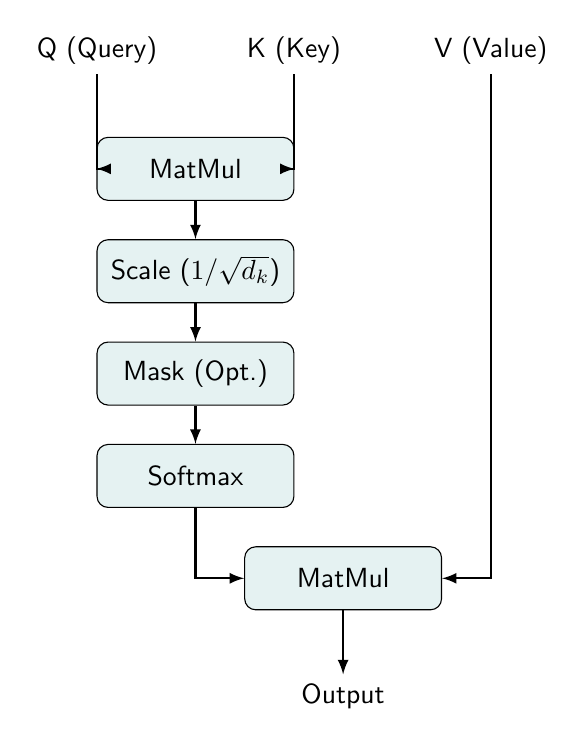
\begin{tikzpicture}[
        op/.style={draw, rectangle, rounded corners, fill=teal!10, minimum width=2.5cm, minimum height=0.8cm, align=center, font=\sffamily},
        data/.style={font=\sffamily},
        arrow/.style={-latex, thick}
    ]
        
        % Data inputs (Absolute positioning)
        \node[data] (q) at (0, 0) {Q (Query)};
        \node[data] (k) at (2.5, 0) {K (Key)};
        \node[data] (v) at (5, 0) {V (Value)};
        
        % Operations (Absolute positioning)
        \node[op] (matmul1) at (1.25, -1.5) {MatMul};
        \node[op] (scale) at (1.25, -2.8) {Scale ($1/\sqrt{d_k}$)};
        \node[op] (mask) at (1.25, -4.1) {Mask (Opt.)};
        \node[op] (softmax) at (1.25, -5.4) {Softmax};
        \node[op] (matmul2) at (3.125, -6.7) {MatMul};
        
        % Output
        \node[data] (out) at (3.125, -8.2) {Output};
        
        % Arrows
        \draw[arrow] (q) |- (matmul1);
        \draw[arrow] (k) |- (matmul1);
        \draw[arrow] (matmul1) -- (scale);
        \draw[arrow] (scale) -- (mask);
        \draw[arrow] (mask) -- (softmax);
        \draw[arrow] (softmax) |- (matmul2);
        \draw[arrow] (v) |- (matmul2);
        \draw[arrow] (matmul2) -- (out);
        
    \end{tikzpicture}
    \caption{缩放点积注意力的数据流图 (Scaled Dot-Product Attention)}
    \label{fig:attention}
\end{figure}

\begin{rosetta}{Self-Attention}
    \begin{equation}
        \text{Attention}(Q, K, V) = \text{softmax}\left(\frac{QK^T}{\sqrt{d_k}}\right)V
    \end{equation}
    其中:
    \begin{itemize}
        \item $Q$ (Query), $K$ (Key), $V$ (Value) 是线性变换后的矩阵。
        \item $d_k$ 是 Key 的维度,除以 $\sqrt{d_k}$ 是为了防止点积结果过大导致梯度消失。
    \end{itemize}
    \tcblower
    \pyfunc{torch.nn.functional.scaled\_dot\_product\_attention}
\end{rosetta}

\section{多头注意力 (Multi-Head Attention)}

多头注意力通过并行运行多个自注意力头,使模型能够同时从不同的表示子空间捕捉信息。

\begin{center}
\begin{tikzpicture}[node distance=1.2cm, font=\sffamily\small]
    % 输入
    \node[data_node] (in) {Input $X$};
    
    % 线型投影
    \node[block, above=0.8cm of in] (proj) {Linear Projections \\ ($W^Q_i, W^K_i, W^V_i$)};
    \draw[conn] (in) -- (proj);
    
    % 多头并行
    \node[attn_block, above left=1cm and 0.5cm of proj] (h1) {Scaled Dot-Product \\ Head 1};
    \node[attn_block, above right=1cm and 0.5cm of proj] (h2) {Scaled Dot-Product \\ Head 2};
    \node[above=0.8cm of proj] (dots) {$\dots$};
    
    \draw[conn] (proj.north) -- (h1.south);
    \draw[conn] (proj.north) -- (h2.south);
    
    % 拼接
    \node[block, above=3cm of proj] (concat) {Concatenation};
    \draw[conn] (h1.north) -- (concat.west);
    \draw[conn] (h2.north) -- (concat.east);
    
    % 输出投影
    \node[block, above=0.8cm of concat] (out_proj) {Linear $W^O$};
    \draw[conn] (concat) -- (out_proj);
    \node[above=0.6cm of out_proj] (out) {Output};
    \draw[conn] (out_proj) -- (out);

    % 背景容器
    \begin{scope}[on background layer]
        \node[container, fit=(h1) (h2) (dots)] (heads_box) {};
        \node[anchor=north east, brandblue!50] at (heads_box.north east) {Multi-Heads};
    \end{scope}
\end{tikzpicture}
\end{center}

\begin{rosetta}{多头注意力计算}
    \begin{equation}
        \text{MultiHead}(Q, K, V) = \text{Concat}(\text{head}_1, \dots, \text{head}_h)W^O
    \end{equation}
    其中 $\text{head}_i = \text{Attention}(QW_i^Q, KW_i^K, VW_i^V)$
    \tcblower
    \pyfunc{nn.MultiheadAttention(embed\_dim, num\_heads)}
\end{rosetta}

\chapter{生成模型数学基础}
\label{ch:generative}

生成模型旨在学习数据的概率分布 $p(x)$,从而生成新的样本。

\section{VAE (Variational Autoencoder)}
VAE 通过最大化变分下界(ELBO)来训练。

\subsection{重参数化技巧 (Reparameterization Trick)}
为了让随机采样过程可导,我们将随机性转移到外部噪声。这使得梯度能够流过分布参数 $\mu$ 和 $\sigma$。

\begin{center}
\begin{tikzpicture}[node distance=1.5cm, font=\sffamily\small]
    % 标准正态噪声
    \node[active_neuron] (eps) {$\epsilon$};
    \node[layer_label, above=0.2cm of eps] {$\mathcal{N}(0, I)$};
    
    % 分布参数
    \node[data_node, left=1.5cm of eps] (mu) {$\mu$};
    \node[data_node, right=1.5cm of eps] (sigma) {$\sigma$};
    
    % 变换操作
    \node[op_node, below=1cm of eps] (mul) {$\times$};
    \node[op_node, below=2cm of eps] (add) {$+$};
    
    \draw[conn] (sigma) |- (mul);
    \draw[conn] (eps) -- (mul);
    \draw[conn] (mul) -- (add);
    \draw[conn] (mu) |- (add);
    
    % 采样结果
    \node[data_node, below=0.8cm of add] (z) {Latent $z$};
    \draw[conn] (add) -- (z);
    
    % 梯度流向标注
    \path[->, >=Stealth, brandorange, dashed, thick] (z.north) edge[bend left=30] node[left] {Gradient Flow} (mu.south);
    \path[->, >=Stealth, brandorange, dashed, thick] (z.north) edge[bend right=30] node[right] {Gradient Flow} (sigma.south);
\end{tikzpicture}
\end{center}

\begin{rosetta}{重参数化}
    \begin{equation}
        \mathbf{z} = \mu + \sigma \odot \epsilon, \quad \epsilon \sim \mathcal{N}(0, I)
    \end{equation}
    \tcblower
    \texttt{z = mu + sigma * torch.randn\_like(sigma)}
\end{rosetta}

\subsection{ELBO 损失函数}
VAE 的目标函数由两部分组成:重建误差和正则化项。

\begin{rosetta}{VAE 损失定义}
    \begin{equation}
        \mathcal{L}_{VAE} = \mathbb{E}_{q(z|x)}[\log p(x|z)] - D_{KL}(q(z|x) \| p(z))
    \end{equation}
    其中第一项是重建似然(通常用 MSE 或 BCE),第二项是隐藏变量分布与先验分布(通常为标准正态)的 KL 散度。
\end{rosetta}

\section{Diffusion Model (扩散模型) 简介}
扩散模型通过逐渐向数据添加噪声(正向过程)和学习去噪(逆向过程)来生成图像。

\begin{center}
\begin{tikzpicture}[node distance=2.5cm, font=\sffamily\small]
    % 状态节点
    \node[data_node, fill=brandblue!10] (x0) {$x_0$};
    \node[data_node, right of=x0] (xt1) {$x_{t-1}$};
    \node[data_node, right of=xt1] (xt) {$x_t$};
    \node[data_node, right of=xt, fill=brandorange!10] (xT) {$x_T$};
    
    % 前向过程 (加噪)
    \draw[data_flow, bend left=25] (x0) to node[above] {$q(x_{t-1}|x_0)$} (xt1);
    \draw[data_flow, bend left=25] (xt1) to node[above] {$q(x_t|x_{t-1})$} (xt);
    \draw[data_flow, bend left=25] (xt) to node[above] {$\dots$} (xT);
    
    % 逆向过程 (去噪)
    \draw[conn, draw=brandorange, bend left=25] (xT) to node[below] {$p_\theta(x_{t-1}|x_t)$} (xt);
    \draw[conn, draw=brandorange, bend left=25] (xt) to node[below] {$\dots$} (xt1);
    \draw[conn, draw=brandorange, bend left=25] (xt1) to node[below] {$p_\theta(x_0|x_1)$} (x0);
    
    % 标签
    \node[layer_label, below=0.3cm of x0] {DATA};
    \node[layer_label, below=0.3cm of xT] {NOISE};
\end{tikzpicture}
\end{center}

\begin{rosetta}{DDPM 正向扩散}
    \begin{equation}
        q(x_t | x_{t-1}) = \mathcal{N}(x_t; \sqrt{1-\beta_t}x_{t-1}, \beta_t I)
    \end{equation}
    通过重参数化,我们可以直接从 $x_0$ 计算 $x_t$。
\end{rosetta}


% --- 第六阶段:大模型纪元 (SOTA) ---
\part{大模型纪元 (Foundation Models)}
\chapter{大模型组件 (LLM Components)}
\label{ch:llm_components}

现代大语言模型(如 LLaMA、Mixtral)在 Transformer 基础架构上引入了更高效的算子,极大增强了模型的外推能力与推理速度。

\section{RMSNorm (Root Mean Square Normalization)}
抛弃了均值平移(Mean-centering),仅使用均方根缩放,从而节省了计算开销而性能基本无损。

\begin{rosetta}{RMSNorm}
    \begin{equation}
        \text{RMSNorm}(x) = \frac{x}{\text{RMS}(x)} \odot \gamma \quad \text{其中 } \text{RMS}(x) = \sqrt{\frac{1}{d} \sum_{i=1}^{d} x_i^2 + \epsilon}
    \end{equation}
    这里 $\gamma$ 是可学习的缩放参数,$\epsilon$ 为防止除零的微小常数。
    \tcblower
    \pyfunc{x / torch.sqrt(torch.mean(x**2) + eps) * weight}
\end{rosetta}

\section{SwiGLU (Swish Gated Linear Unit)}
LLaMA 中的默认激活机制,采用 Swish 变体控制信息流。

\begin{rosetta}{SwiGLU}
    \begin{equation}
        \text{SwiGLU}(x, W, V) = \text{Swish}(xW) \odot xV
    \end{equation}
    \textbf{其中 Swish 函数定义为}:
    \begin{equation}
        \text{Swish}_{\beta}(z) = z \cdot \sigma(\beta z) = \frac{z}{1 + e^{-\beta z}}
    \end{equation}
    当 $\beta=1$ 时,即为 SiLU 函数。
\end{rosetta}

\section{RoPE (Rotary Position Embedding)}
旋转位置编码通过将绝对位置注入为旋转矩阵,自然推导出了相对位置衰减特性。

\begin{rosetta}{RoPE (旋转位置编码)}
    对于位置 $m$ 的特征向量 $\mathbf{x} = [x_1, x_2, \dots, x_{d}]$,将其两两分组应用旋转矩阵:
    \begin{equation}
        f(\mathbf{x}, m) = \mathbf{x} R_{\Theta, m}^d
    \end{equation}
    \textbf{旋转矩阵 $R_{\Theta, m}^d$}:
    \begin{equation}
        \begin{bmatrix}
            \cos m\theta_1 & -\sin m\theta_1 & 0 & 0 & \dots \\
            \sin m\theta_1 & \cos m\theta_1 & 0 & 0 & \dots \\
            0 & 0 & \cos m\theta_2 & -\sin m\theta_2 & \dots \\
            0 & 0 & \sin m\theta_2 & \cos m\theta_2 & \dots \\
            \vdots & \vdots & \vdots & \vdots & \ddots
        \end{bmatrix}
    \end{equation}
    其中基频 $\theta_i = 10000^{-2(i-1)/d}$。
\end{rosetta}

\section{MoE (Mixture of Experts)}
通过路由机制(Routing)让每个 Token 仅激活部分参数(如 Top-2),实现参数量扩大而不增加前向推理时间。

\begin{rosetta}{Top-K 路由数学}
    \textbf{路由权重}: 对于输入 $x$,专家 $E_i$ 的权重为:
    \begin{equation}
        G(x)_i = \begin{cases}
            \frac{e^{x \cdot W_{r, i}}}{\sum_{j \in T} e^{x \cdot W_{r, j}}}, & \text{if } i \in T \\
            0, & \text{otherwise}
        \end{cases}
    \end{equation}
    其中 $T$ 是根据 $x \cdot W_r$ 选出的 Top-K 索引集合。
    
    \textbf{最终输出}:
    \begin{equation}
        y = \sum_{i=1}^{N} G(x)_i E_i(x)
    \end{equation}
\end{rosetta}

\chapter{状态空间模型 (SSM \& Mamba)}
\label{ch:ssm_mamba}

状态空间模型(State Space Models,如 S4、Mamba)是试图替代 Transformer 作为序列建模基石的架构,它结合了 RNN 的推理效率和 CNN 的训练并行性。

\section{连续系统数学模型 (ODE)}

\begin{variable}
\begin{itemize}
    \item $h(t) \in \mathbb{R}^N$: 隐藏状态,代表系统的记忆,$N$ 为状态维度。
    \item $\mathbf{A} \in \mathbb{R}^{N \times N}$: 演化矩阵,控制记忆的衰减与转换。
    \item $\mathbf{B} \in \mathbb{R}^{N \times 1}$: 输入矩阵,将一维输入映射到 $N$ 维状态空间。
    \item $\mathbf{C} \in \mathbb{R}^{1 \times N}$: 输出矩阵,将状态空间重新映射回输出信号。
    \item $\Delta$: 离散化步长,控制采样的时间密度。
\end{itemize}
\end{variable}

状态空间模型本质上是将输入信号 $x(t) \in \mathbb{R}$ 映射到隐藏状态 $h(t) \in \mathbb{R}^N$,再投影到输出 $y(t) \in \mathbb{R}$ 的常微分方程。

\begin{rosetta}{连续域常微分方程}
    \textbf{状态方程}:
    \begin{equation}
        h'(t) = \mathbf{A}h(t) + \mathbf{B}x(t)
    \end{equation}
    \textbf{输出方程}:
    \begin{equation}
        y(t) = \mathbf{C}h(t) + \mathbf{D}x(t)
    \end{equation}
    其中 $\mathbf{A} \in \mathbb{R}^{N \times N}$ 是演化矩阵,通常使用 HiPPO(High-order Polynomial Projection Operators)初始化,以确保系统能够“记住”历史。
\end{rosetta}

\section{离散化 (Discretization: ZOH)}

在实际的深度学习处理中,信号是离散的文本 Token(时间间隔 $\Delta$)。我们需要使用零阶保持(Zero-Order Hold, ZOH)将其离散化为类似 RNN 的差分方程形式。

\begin{rosetta}{ZOH 离散变换}
    给定步长 $\Delta$,离散系统参数 $\bar{\mathbf{A}}$ 和 $\bar{\mathbf{B}}$ 的严格数学推导为:
    \begin{align}
        \bar{\mathbf{A}} &= \exp(\Delta \mathbf{A}) \\
        \bar{\mathbf{B}} &= (\Delta \mathbf{A})^{-1} (\exp(\Delta \mathbf{A}) - I) \cdot \Delta \mathbf{B}
    \end{align}
    \textbf{离散递推公式}:
    \begin{align}
        h_k &= \bar{\mathbf{A}}h_{k-1} + \bar{\mathbf{B}}x_k \\
        y_k &= \mathbf{C}h_k
    \end{align}
    *(省略 D 项,通常在网络中视为残差连接。)*
\end{rosetta}

\section{选择性扫描 (Mamba: Selective Scan)}

在传统的 S4 中,$\bar{\mathbf{A}}, \bar{\mathbf{B}}$ 对于所有时间步是**时不变的(LTI)**,因此可以通过 FFT(快速傅里叶变换)进行卷积加速。
而 Mamba 的核心突破在于**数据相关性(Data-Dependent)**:让 $\Delta, \mathbf{B}, \mathbf{C}$ 成为输入 $x_t$ 的函数,从而能够选择性地过滤或记住信息(类似于 LSTM 的遗忘门)。

\begin{center}
\begin{tikzpicture}[node distance=1.5cm, font=\sffamily\small]
    % 输入
    \node[data_node] (x) {$x_t$};
    
    % 参数生成
    \node[block, right=1.5cm of x] (linear_delta) {$\text{Linear}_{\Delta}$};
    \node[block, above=0.5cm of linear_delta] (linear_b) {$\text{Linear}_{B}$};
    \node[block, below=0.5cm of linear_delta] (linear_c) {$\text{Linear}_{C}$};
    
    \draw[conn] (x) -- (linear_delta);
    \draw[conn] (x) |- (linear_b);
    \draw[conn] (x) |- (linear_c);
    
    % 生成的参数
    \node[active_neuron, right=1cm of linear_delta] (delta) {$\Delta_t$};
    \node[active_neuron, right=1cm of linear_b] (bt) {$B_t$};
    \node[active_neuron, right=1cm of linear_c] (ct) {$C_t$};
    
    \draw[data_flow] (linear_delta) -- (delta);
    \draw[data_flow] (linear_b) -- (bt);
    \draw[data_flow] (linear_c) -- (ct);
    
    % SSM 核心
    \node[block, right=1.5cm of delta, fill=brandblue!20] (ssm) {Selective SSM \\ $h_t = \bar{A}h_{t-1} + \bar{B}x_t$};
    \draw[conn] (delta) -- (ssm);
    \draw[conn] (bt) -| (ssm);
    \draw[conn] (ct) -| (ssm);
    \draw[conn] (x) -- ++(0,-2) -| (ssm);

    % 背景容器
    \begin{scope}[on background layer]
        \node[container, fit=(linear_delta) (linear_b) (linear_c) (delta) (bt) (ct)] (selection_logic) {};
        \node[anchor=south west, brandorange!50] at (selection_logic.north west) {Selection Mechanism};
    \end{scope}
\end{tikzpicture}
\end{center}

\begin{rosetta}{Mamba 选择性机制}
    由于时变特性,FFT 不再适用。Mamba 使用高效的前缀和扫描算法(Hardware-aware Scan):
    \begin{equation}
        \mathbf{B}_t = \text{Linear}_{B}(x_t), \quad \mathbf{C}_t = \text{Linear}_{C}(x_t)
    \end{equation}
    \begin{equation}
        \Delta_t = \text{Softplus}(\text{Linear}_{\Delta}(x_t))
    \end{equation}
    此时 $h_t$ 的递推变为时变的:
    \begin{equation}
        h_t = \bar{\mathbf{A}}_t h_{t-1} + \bar{\mathbf{B}}_t x_t
    \end{equation}
\end{rosetta}

\chapter{参数高效微调 (PEFT \& LoRA)}
\label{ch:peft_lora}

当模型规模增长至百亿甚至千亿参数时,全参微调(Full Fine-Tuning)的显存和计算成本难以承受。低秩自适应(Low-Rank Adaptation, LoRA)通过极少的额外参数,保留了原始知识并适应新任务。

\begin{notation}
\begin{itemize}
    \item $x$: Input tensor
    \item $y$: Output label
    \item $W$: Weight matrix
    \item $\sigma$: Activation function
    \item $\mathbf{x}$: Input vector
    \item $h$: Hidden state
\end{itemize}
\end{notation}

\mnote{$x$: Input tensor \\ $y$: Output label \\ $W$: Weight matrix \\ $\sigma$: Activation function \\ $\mathbf{x}$: Input vector}
\mnote{$h$: Hidden state}
\section{矩阵低秩分解}

LoRA 的核心思想是冻结预训练模型的权重矩阵,并通过旁路的两个低秩矩阵之积来表示权重的增量($\Delta W$)。

\begin{center}
\begin{tikzpicture}[node distance=1.5cm, font=\sffamily\small]
    % 输入
    \node (x) at (0,0) {$x \in \mathbb{R}^k$};
    
    % 主路径:冻结权重
    \node[block, above=1cm of x, minimum height=3cm, fill=brandblue!10] (w0) {Frozen Pretrained \\ $W_0 \in \mathbb{R}^{d \times k}$};
    \draw[conn] (x) -- (w0);
    
    % 旁路:LoRA 路径
    \node[data_node, right=2cm of w0] (matA) {$A \in \mathbb{R}^{r \times k}$};
    \node[data_node, above=1.5cm of matA] (matB) {$B \in \mathbb{R}^{d \times r}$};
    
    \draw[conn] (x.east) -- ++(1,0) |- (matA.west);
    \draw[conn] (matA) -- node[right, math_text] {rank $r \ll d, k$} (matB);
    
    % 合并
    \node[op_node, above=4.5cm of x] (sum) {$+$};
    \draw[conn] (w0) -- (sum);
    \draw[conn] (matB) |- (sum);
    
    % 输出
    \node[above=0.8cm of sum] (out) {$h = W_0 x + BAx$};
    \draw[conn] (sum) -- (out);

    % 标注
    \begin{scope}[on background layer]
        \node[container, fit=(matA) (matB)] (lorabox) {};
        \node[anchor=south west, brandorange] at (lorabox.north west) {Trainable LoRA};
    \end{scope}
\end{tikzpicture}
\end{center}

\begin{rosetta}{LoRA 更新公式}
    设预训练权重矩阵为 $W_0 \in \mathbb{R}^{d \times k}$,冻结不变。
    更新量 $\Delta W$ 通过两个低秩矩阵 $B \in \mathbb{R}^{d \times r}$ 和 $A \in \mathbb{R}^{r \times k}$ 乘积得到:
    \begin{equation}
        W = W_0 + \Delta W = W_0 + B A
    \end{equation}
    其中秩 $r \ll \min(d, k)$,例如 $r=8$ 或 $r=64$。
\end{rosetta}

\section{前向传播与初始化}

\subsection{前向计算逻辑}
对于输入 $\mathbf{x} \in \mathbb{R}^k$,全连接层的原本输出为 $h = W_0 \mathbf{x}$。引入 LoRA 之后,前向传播变为两个并行的矩阵乘法最后相加。

\begin{rosetta}{LoRA 前向传播}
    \begin{equation}
        h = W_0 \mathbf{x} + \frac{\alpha}{r} B A \mathbf{x}
    \end{equation}
    其中 $\alpha$ 是一个缩放超参数,在初始阶段控制新加入参数对最终结果的影响。当秩 $r$ 改变时,可以通过 $\frac{\alpha}{r}$ 保持方差稳定。
    \tcblower
    \pyfunc{y = F.linear(x, W0) + F.linear(x, B @ A) * (alpha / r)}
\end{rosetta}

\subsection{零初始化技巧}
为了保证在训练刚开始时(即第一个 Step 前),引入的 LoRA 模块不会破坏预训练模型的行为,矩阵 $A$ 和 $B$ 的初始化至关重要。

\begin{rosetta}{LoRA 初始化}
    \textbf{矩阵 A}: 使用标准正态分布初始化(Gaussian / Kaiming)。
    \begin{equation}
        A \sim \mathcal{N}(0, \sigma^2)
    \end{equation}
    \textbf{矩阵 B}: 必须使用全零矩阵初始化。
    \begin{equation}
        B = \mathbf{0} \implies B A = \mathbf{0}
    \end{equation}
    这样,初始状态下 $\Delta W = 0$,保证了 $h = W_0 \mathbf{x}$ 与原始模型输出完全一致。
\end{rosetta}

\section{推理合并 (Merging Weights)}

在推理阶段,由于矩阵乘法的分配律,我们可以直接将 $BA$ 加回到 $W_0$ 中。因此,部署带有 LoRA 的大模型,其**推理延迟与基座模型完全相同**(Zero Latency Cost)。

\begin{rosetta}{LoRA 部署公式}
    \begin{equation}
        W_{deploy} = W_0 + B A
    \end{equation}
    在 PyTorch 中只需执行 \pyfunc{W0.add\_(B @ A)} 即可卸载独立参数。
\end{rosetta}


% --- 第七阶段:前沿探索 (The Frontiers) ---
\part{前沿探索 (The Frontiers)}
\chapter{对抗与对比学习}
\label{ch:adversarial_contrastive}

传统的预测任务旨在最小化误差,而对抗与对比学习则是让模型在数据分布与表征空间中互相博弈或聚类。

\section{生成对抗网络 (GAN)}
GAN 由生成器 (Generator) 和判别器 (Discriminator) 组成,两者进行极小极大博弈 (Min-Max Game)。

\begin{rosetta}{GAN 目标函数}
    \begin{equation}
        \min_G \max_D V(D, G) = \mathbb{E}_{x \sim p_{data}}[\log D(x)] + \mathbb{E}_{z \sim p_z}[\log(1 - D(G(z)))]
    \end{equation}
    判别器 $D$ 试图将原数据打高分 (1),假数据打低分 (0);生成器 $G$ 试图骗过 $D$(让 $D(G(z))$ 趋近于 1)。
\end{rosetta}

\section{对比学习与 InfoNCE 损失}
多模态模型(如 CLIP)和自监督学习的核心,通过拉近正样本、推开负样本来学习高维特征。

\begin{rosetta}{InfoNCE (Temperature Scaled Cross-Entropy)}
    \begin{equation}
        \mathcal{L}_q = -\log \frac{\exp(\mathbf{q} \cdot \mathbf{k}^+ / \tau)}{\sum_{i=0}^{K} \exp(\mathbf{q} \cdot \mathbf{k}_i / \tau)}
    \end{equation}
    其中 $\mathbf{q}$ 是查询向量,$\mathbf{k}^+$ 是匹配的正样本,$\tau$ 是温度超参数(控制对困难负样本的惩罚力度)。
    \tcblower
    \pyfunc{F.cross\_entropy(logits / temperature, labels)}
\end{rosetta}

\chapter{图网络与空间视觉}
\label{ch:graph_vision}

超越传统的网格数据(像素),神经网络能够处理非欧几里得空间(图)或以全新视角审视视觉(Patch)。

\begin{notation}
\begin{itemize}
    \item $x$: Input tensor
    \item $W$: Weight matrix
    \item $\sigma$: Activation function
    \item $\mathbf{x}$: Input vector
\end{itemize}
\end{notation}

\mnote{$x$: Input tensor \\ $W$: Weight matrix \\ $\sigma$: Activation function \\ $\mathbf{x}$: Input vector}
\section{图卷积网络 (GCN)}
在图数据上进行信息传递(Message Passing),节点特征通过邻接矩阵进行聚合。

\begin{rosetta}{GCN 谱图聚合规则}
    \begin{equation}
        H^{(l+1)} = \sigma\left(\tilde{D}^{-\frac{1}{2}} \tilde{A} \tilde{D}^{-\frac{1}{2}} H^{(l)} W^{(l)}\right)
    \end{equation}
    其中:
    \begin{itemize}
        \item $\tilde{A} = A + I_N$ 是带有自环的邻接矩阵(即每个节点也看自己)。
        \item $\tilde{D}$ 是 $\tilde{A}$ 的度矩阵(对角阵,用于归一化,防止度大的节点梯度爆炸)。
        \item $H^{(l)}$ 是第 $l$ 层的节点特征矩阵。
    \end{itemize}
\end{rosetta}

\section{视觉 Transformer (ViT)}
将图像视为序列 (Sequence of Patches),彻底打破了 CNN 的归纳偏置。

\begin{rosetta}{ViT Patch 嵌入}
    一张 $H \times W \times C$ 的图像被切割为 $N$ 个大小为 $P \times P$ 的图像块。
    \begin{equation}
        N = \frac{H \times W}{P^2}
    \end{equation}
    \textbf{数学展开}:
    \begin{equation}
        \mathbf{z}_0 = [x_{\text{class}}; \, \mathbf{x}_p^1\mathbf{E}; \, \dots; \, \mathbf{x}_p^N\mathbf{E}] + \mathbf{E}_{pos}
    \end{equation}
    其中 $\mathbf{x}_p^i$ 是展平的图像块,$\mathbf{E}$ 是线性投影矩阵,$\mathbf{E}_{pos} \in \mathbb{R}^{(N+1) \times D}$ 是可学习的 1D 位置编码,$x_{\text{class}}$ 是用于分类的全局 Token。
\end{rosetta}

\chapter{对齐与极端量化}
\label{ch:alignment_quantization}

当大模型具备涌现能力后,下一步是让其输出符合人类偏好(对齐),并能在消费级硬件上运行(量化)。

\begin{notation}
\begin{itemize}
    \item $y$: Output label
    \item $\theta$: Model parameters
    \item $\sigma$: Activation function
\end{itemize}
\end{notation}

\mnote{$y$: Output label \\ $\theta$: Model parameters \\ $\sigma$: Activation function}
\section{直接偏好优化 (DPO)}
彻底绕过了传统 RLHF 中复杂的强化学习 (PPO) 训练流程,直接在偏好数据上优化语言模型本身。

\begin{rosetta}{DPO 目标函数}
    设 $\pi_\theta$ 为正在训练的模型,$\pi_{ref}$ 为参考模型,$y_w$ 为人类偏好的回答,$y_l$ 为被拒绝的回答。
    \begin{equation}
        \mathcal{L}_{DPO} = -\mathbb{E}_{(x, y_w, y_l)} \left[ \log \sigma \left( \beta \log \frac{\pi_\theta(y_w|x)}{\pi_{ref}(y_w|x)} - \beta \log \frac{\pi_\theta(y_l|x)}{\pi_{ref}(y_l|x)} \right) \right]
    \end{equation}
    其中 $\beta$ 是控制偏离参考模型程度的温度系数,$\sigma$ 为 Sigmoid 函数。该公式隐式定义了奖励。
\end{rosetta}

\section{QLoRA 与 NF4 量化}
为了在单张显卡上微调大模型,QLoRA 引入了一种信息论上最优的新数据类型:4-bit NormalFloat (NF4)。

\begin{rosetta}{分位数归一化与双重量化}
    \textbf{NF4 的数学基础}:
    假设神经网络的权重服从均值为 0 的正态分布 $\mathcal{N}(0, \sigma^2)$。NF4 预先计算了该分布的 16 个等概率分位数作为量化点.
    \begin{equation}
        q_i = \frac{1}{2} \left( Q\left(\frac{i}{16}\right) + Q\left(\frac{i+1}{16}\right) \right)
    \end{equation}
    \textbf{双重量化 (Double Quantization)}: 
    为了存储量化所需的缩放常数 $c$,对这些常数进行二次 8-bit 量化,使得平均每参数的内存开销再降低 $0.37$ bits。
\end{rosetta}

\chapter{下一代生成法则}
\label{ch:nextgen_generative}

超越经典的 VAE 与基础扩散模型,当代生成大模型(图像、视频)采用了更强大的引导机制与流模型数学框架。

\begin{notation}
\begin{itemize}
    \item $x$: Input tensor
    \item $\theta$: Model parameters
\end{itemize}
\end{notation}

\mnote{$x$: Input tensor \\ $\theta$: Model parameters}
\section{无分类器引导 (CFG - Classifier-Free Guidance)}
Stable Diffusion 系列模型“听懂”人类 Prompt 的绝对核心数学技巧。

\begin{rosetta}{CFG 向量外插}
    在每个去噪步 $t$,模型同时预测有条件(Prompt $c$)和无条件(空文本 $\emptyset$)的噪声。
    \begin{equation}
        \hat{\epsilon}_\theta(x_t, c) = \epsilon_\theta(x_t, \emptyset) + w \cdot \left( \epsilon_\theta(x_t, c) - \epsilon_\theta(x_t, \emptyset) \right)
    \end{equation}
    其中 $w$ 即为 \texttt{guidance\_scale}。当 $w > 1$ 时,它在几何空间中强行放大了向条件 $c$ 靠近的方向向量,从而生成高度匹配 Prompt 但可能略微降低多样性的图像。
\end{rosetta}

\section{流匹配与整流 (Flow Matching \& Rectified Flows)}
Sora 和 Stable Diffusion 3 抛弃了传统的 DDPM 马尔可夫链,转向基于连续常微分方程 (ODE) 的直接轨迹预测。

\begin{rosetta}{Rectified Flows (ODE)}
    建立一条从纯噪声 $X_0 \sim \mathcal{N}(0, I)$ 到真实数据 $X_1$ 的直线轨迹:
    \begin{equation}
        X_t = t X_1 + (1 - t) X_0, \quad t \in [0, 1]
    \end{equation}
    神经网络 $v_\theta(X_t, t)$ 的目标是直接预测这条直线的导数(即流场):
    \begin{equation}
        \mathcal{L} = \mathbb{E}_{t, X_0, X_1} \left[ \| v_\theta(X_t, t) - (X_1 - X_0) \|_2^2 \right]
    \end{equation}
    这比扩散模型试图预测加入的随机噪声在数学上更加优美,且在采样时能以极少的步数求得 ODE 积分。
\end{rosetta}


\backmatter
\bibliographystyle{plainnat}
\bibliography{references}

\end{document}
